\section{\SystemName Design}

\noindent\textbf{Overview of \SystemName's Design.}
\SystemName is designed to answer one question: what quantum hardware speed is required for a quantum-circuit application to beat the native HPC application for the same task? Figure~\ref{fig:design-overview} summarizes the key components. First, \SystemName uses \textit{Shared Workload Control} to ensure that all paths use the same input instance and quality target. Second, it uses \textit{Native Path Execution} to establish a strong classical baseline. Third, it uses \textit{Quantum Path Execution} to run quantum kernels, QNN/VQC, VQE, QAOA, and Hamiltonian simulation circuits with \cuQuantum. Finally, it uses \textit{Supremacy Threshold Analysis} to estimate the future quantum hardware requirements.

\noindent\textbf{Design Boundary.}
\SystemName is not a new quantum circuit simulator, compiler, or quantum algorithm. It treats existing simulators and native methods as execution engines behind a controlled workload interface. The design contribution is the measurement discipline: same input, same quality metric, strongest valid native path, measured quantum-circuit path, and explicit hardware projection. This boundary is important because faster simulation alone does not answer whether a future quantum computer would beat the native application.

\begin{figure}[t]
    \centering
    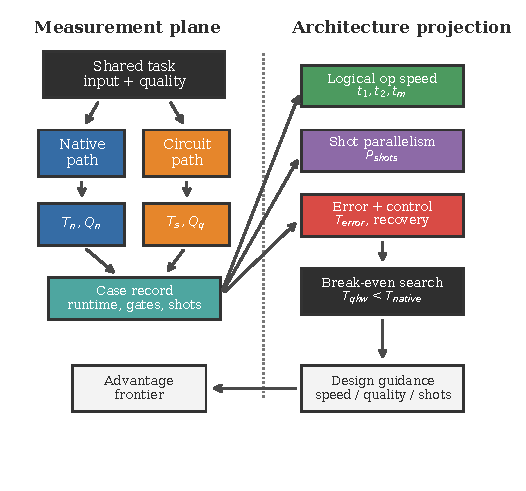
\includegraphics[width=\linewidth]{figures/design_overview.pdf}
    \Description{Block diagram of QSupremacy with shared workload control, native path execution, quantum path execution, measurement logging, and supremacy threshold analysis.}
    \caption{Architecture and procedure of \SystemName.}
    \label{fig:design-overview}
\end{figure}

\subsection{Overall Procedure}

Figure~\ref{fig:design-overview} shows the overall procedure. \SystemName has two main phases: \textit{Measurement} and \textit{Supremacy Analysis}.

\noindent\textbf{Measurement.}
When an experiment starts, \SystemName reads the workload configuration. The configuration includes the dataset, train/test split, feature dimension, model type, circuit type, shots, and target quality. \SystemName then runs the native path and the quantum-circuit path using the same input data. This prevents unfair comparisons caused by different preprocessing or different quality targets.

\noindent\textbf{Config Record.}
Before any path is executed, \SystemName materializes a single configuration record. This record is the logical owner of the experiment. It stores the workload family, instance ID, random seed, feature transform, native candidates, quantum circuit family, circuit depth, shot setting, and quality metric. The native and quantum paths do not choose these values independently. They receive the same record and append path-specific measurements to it. This mirrors the task-oriented style in the previous papers: the system first creates a stable representation of the work, then later components operate on that representation.

\noindent\textbf{Supremacy Analysis.}
After measurement, \SystemName reads the circuit metadata and runtime breakdown. It extracts the number of qubits, circuit depth, one-qubit gates, two-qubit gates, shots, and optimizer iterations. Using this information, \SystemName computes the quantum hardware speed required to make the projected quantum path faster than the measured native path.

\noindent\textbf{Failure Handling.}
\SystemName treats failed paths as measurement results rather than silently dropping them. If a native candidate fails, the record keeps the error and continues with other native candidates. If a quantum path fails, the record keeps the circuit metadata available up to the failure point and marks the case as non-advantaged. This rule is important for large sweeps because feasibility is part of the systems question. A workload that only succeeds after removing difficult cases would overstate the advantage frontier.

\subsection{Shared Workload Control}

\noindent\textbf{Dataset Control.}
\SystemName first fixes the workload. The first full workload is \texttt{sklearn digits}. \SystemName uses a fixed train/test split and applies PCA to 4, 8, 12, and 16 dimensions. The same reduced features are used by every native and quantum model.

\noindent\textbf{Instance Identity.}
Each measured case receives a deterministic identity. For ML, the identity includes the class pair, sample count, PCA dimension, circuit depth, and seed. For chemistry, it includes the molecule, basis, active-space setting, and circuit layer count. For optimization, it includes the graph family, graph size, seed, and QAOA layer count. For simulation, it includes the Hamiltonian model, number of qubits, evolution time, and approximation setting. This identity is used in filenames, JSON records, summaries, and paper figures. As a result, a figure bar can be traced back to the exact raw case that produced it.

\noindent\textbf{Application Control.}
\SystemName then extends the same rule to practical workloads. For drug discovery, the native path may be a classical molecular simulation or learned surrogate, while the quantum path may be a VQE-style molecular energy circuit. For optimization, the native path may be a mixed-integer, local-search, or GPU heuristic baseline, while the quantum path may be a QAOA-style circuit. For simulation, the native path may be a classical numerical solver, while the quantum path may be a Hamiltonian simulation circuit. In every case, \SystemName keeps the task, input instance, output metric, and quality target fixed.

\noindent\textbf{Quality Control.}
\SystemName defines the target quality before execution. The target can be a fixed accuracy threshold or a time-to-best-quality curve. This is important because a quantum path with lower accuracy cannot be claimed faster than a native path with higher accuracy.

\noindent\textbf{Quality Normalization.}
Different application families expose different quality values, so \SystemName stores both the native metric and a normalized gap. For classification, the gap is based on accuracy. For chemistry, it is based on energy error relative to the native reference. For optimization, it is based on objective gap. For simulation, it is based on state or observable error. The normalized gap lets the threshold analysis ask a common question across families: how much of the quality gap must future quantum hardware and algorithms recover before runtime speed becomes relevant?

\noindent\textbf{Why This Matters.}
Without shared workload control, the comparison becomes ambiguous. A native model may use a different feature dimension or a different split from the quantum model. \SystemName avoids this by making the workload controller the first step in the pipeline.

\subsection{Application Path Execution}

\subsubsection{Native Path Execution}

\noindent\textbf{Classical Baselines.}
The native path executes the best available non-quantum implementation for the same input. For ML, \SystemName supports softmax regression, MLP, linear ridge classification, RBF kernel ridge classification, k-nearest neighbors, and nearest-centroid baselines without requiring an external ML package. For chemistry, the native path computes molecular energy from the same Hamiltonian by exact dense diagonalization and, in the strengthened implementation, sparse Lanczos/eigensolver baselines for Pauli Hamiltonians. For optimization, \SystemName records exact enumeration when feasible and also greedy, local-search, and simulated-annealing baselines. For scientific simulation, the native path includes dense exact time evolution and a sparse Krylov-style evolution baseline. The native time used in the threshold is the fastest implemented model that reaches the best native quality within a small tolerance. This rule prevents a weak or low-quality native model from making the quantum path look artificially competitive.

\noindent\textbf{Runtime Breakdown.}
\SystemName records preprocessing time, training time, inference time, and total time. It also records accuracy and model metadata. These values define $T_{\mathrm{native}}$, which is the target that the projected quantum hardware path must beat.

\noindent\textbf{Baseline Selection Rule.}
The native path may produce several valid answers for one case. \SystemName first removes candidates that do not meet the family-specific quality rule. Among the remaining candidates, it selects the fastest one as the native baseline. If no native candidate reaches the quality target, the best-quality native candidate is still recorded, but the case is marked so that the threshold analysis does not create an artificial win. This selection rule is deliberately conservative: adding a stronger native method can only make the quantum threshold harder, not easier.

\subsubsection{Quantum Kernel Path}

\noindent\textbf{Feature Map Execution.}
The quantum kernel path maps each PCA feature vector into a quantum feature map. \cuQuantum simulates the circuit and produces state or observable data for kernel entries. A classical classifier then consumes the kernel matrix.

\noindent\textbf{Cost Breakdown.}
\SystemName records encoding time, circuit construction time, \cuQuantum execution time, kernel matrix construction time, and classifier-head time. This path is useful because it separates circuit execution cost from trainable quantum-parameter optimization.

\noindent\textbf{Expected Bottleneck.}
The kernel path can become expensive because the kernel matrix grows with the number of samples. Therefore, \SystemName must report both sample scaling and feature-dimension scaling.

\noindent\textbf{Kernel Accounting Rule.}
The kernel path is counted at the application level, not only at the circuit-kernel level. \SystemName records how many pairwise circuit evaluations are required, how many are actually executed, whether symmetry is used, and how the resulting matrix is consumed by the classifier. This matters because a circuit that is fast for one encoded sample can still be expensive after all sample pairs are evaluated. The design therefore exposes the sample-count multiplier instead of hiding it inside one aggregate runtime.

\subsubsection{QNN/VQC Path}

\noindent\textbf{Parameterized Circuit Execution.}
The QNN/VQC path maps the same PCA features into a parameterized quantum circuit. It then updates trainable parameters through a classical optimizer. Each optimizer step can require many circuit evaluations.

\noindent\textbf{Cost Breakdown.}
\SystemName records ansatz type, depth, gate count, number of parameters, optimizer iterations, observable extraction time, and accuracy. This path is expected to be more expensive than the quantum kernel path because training repeatedly evaluates the circuit.

\noindent\textbf{Why This Matters.}
QNN/VQC models are often discussed as quantum machine-learning candidates. However, their systems cost is easy to underestimate. \SystemName makes the repeated circuit evaluations visible.

\noindent\textbf{Optimizer Rule.}
For variational paths, \SystemName records the outer-loop optimizer separately from circuit execution. The record includes the number of parameter vectors, the number of observables, the number of shots per evaluation, and the measured time spent outside \cuQuantum. This separation is needed because future quantum hardware can reduce circuit execution time without removing the classical optimizer loop. If the optimizer or data movement dominates, the projected hardware speedup has limited effect.

\subsection{Measurement and Threshold Analysis}

\noindent\textbf{JSON Record.}
Every run emits a JSON record. The record includes dataset metadata, model metadata, runtime breakdowns, accuracy, circuit qubits, circuit depth, gate counts, shots, GPU metadata, and Slurm metadata where available.

\noindent\textbf{Summary Path.}
\SystemName keeps raw case records separate from derived summaries. A sweep first writes one JSON object per case or per task shard. A summarizer then validates expected case counts, merges shards, computes medians and quantiles, and writes CSV/JSON summaries used by the figures. The paper audit reads these summaries and checks that the claims in the manuscript match the stored values. This design follows the same spirit as prior systems papers: the evaluation does not depend on hand-copied numbers.

\noindent\textbf{Allocation Accounting.}
\SystemName separates login-node smoke tests from Slurm performance runs. Login-node tests are only for correctness. Slurm runs must record elapsed time, queue time, requested walltime, allocated GPUs, and charged node-hours. This prevents short sanity checks from being mistaken for valid performance experiments.

\subsubsection{Threshold Analysis}

\noindent\textbf{Execution Model.}
Given circuit metadata, \SystemName estimates projected quantum execution time:

\begin{align}
T_{\mathrm{execute}} =
\frac{N_s(D_1t_1 + D_2t_2 + D_mt_m)}
{P_{\mathrm{shots}}}
+ T_{\mathrm{error}},
\end{align}

where $N_s$ is the shot count, $D_1$ and $D_2$ are one- and two-qubit gate depths, $D_m$ is measurement depth, $t_1$, $t_2$, and $t_m$ are logical operation times, and $P_{\mathrm{shots}}$ is shot-level parallelism.

\noindent\textbf{Break-even Search.}
\SystemName inverts the model. Instead of assuming a quantum speedup, it asks what logical gate time, shot throughput, and error overhead are needed for:

\begin{align}
T_{\mathrm{qhw}} < T_{\mathrm{native}}.
\end{align}

This gives a hardware requirement rather than a vague claim of supremacy.

\noindent\textbf{Advantage Frontier.}
\SystemName does not reduce the result to one speedup number. It sweeps hardware assumptions and reports the feasible region where the projected quantum path beats the native path at the same quality. This region is the advantage frontier. If no reasonable region exists, the workload is classified by the limiting factor: quality, encoding, shots, error overhead, or native baseline strength.

\noindent\textbf{Frontier Classification.}
After the sweep, each case is assigned a primary limiting factor. A case is speed-limited when quality is close enough but the required runtime improvement is large. It is quality-limited when even aggressive speedup does not help unless the output gap closes. It is encoding- or shot-limited when non-kernel overhead dominates the projection. It is native-dominated when a strong native baseline makes the required improvement much larger than the quantum path can plausibly recover. This classification turns the frontier into a diagnostic result instead of only a plot.

\subsection{Advantage Claim Checklist}

A practical quantum-advantage claim should pass a small set of systems checks before it is treated as meaningful. Table~\ref{tab:claim-checklist} lists the checks used by \SystemName. The checklist is intentionally strict because a weak native baseline, a different input instance, or a lower-quality quantum output can all create a false impression of advantage.

\begin{table}[t]
\caption{Checklist for a practical quantum-advantage claim.}
\centering
\small
\resizebox{\columnwidth}{!}{%
\begin{tabular}{lll}
\toprule
\textbf{Check} & \textbf{Question} & \textbf{\SystemName evidence} \\
\midrule
Same task & Are native and quantum paths solving the same input? & Shared workload config \\
Same quality & Does the quantum path meet the native target? & Accuracy, energy, objective, observable gap \\
Strong native & Is the native path the fastest valid baseline? & Baseline selection rule \\
End-to-end cost & Are encoding, execution, measurement, and postprocess included? & Runtime breakdown and metadata \\
Hardware projection & What future quantum speed is required? & Required speedup and frontier \\
Error/shot overhead & Could shots or error correction erase speedup? & Projection parameters and sensitivity \\
Repeatability & Can the result be regenerated on the system? & Slurm scripts, summaries, accounting \\
\bottomrule
\end{tabular}
}
\label{tab:claim-checklist}
\end{table}

\subsection{Workload Suite}

Table~\ref{tab:workload-suite} shows the measured workload suite. The digits workload is the controlled calibration case. The practical suite covers the application families that motivate many real-world quantum-computing claims.

\begin{table}[t]
\caption{Measured workload suite.}
\centering
\small
\resizebox{\columnwidth}{!}{%
\begin{tabular}{llll}
\toprule
\textbf{Family} & \textbf{Native path} & \textbf{Quantum path} & \textbf{Quality target} \\
\midrule
ML classification & Logistic/MLP/SVM & Kernel, QNN/VQC & Accuracy, loss \\
Drug discovery & Classical energy/surrogate & VQE energy circuit & Energy error, rank quality \\
Optimization & MILP/heuristic/GPU search & QAOA circuit & Objective gap \\
Scientific simulation & Classical solver & Hamiltonian simulation & State/error metric \\
\bottomrule
\end{tabular}
}
\label{tab:workload-suite}
\end{table}
